%%%%%%%%%%%%%%%%%%%%%%%%%%%%%%%%%%%%%%%%%
% Structured General Purpose Assignment
% LaTeX Template
%
% This template has been downloaded from:
% http://www.latextemplates.com
%
% Original author:
% Ted Pavlic (http://www.tedpavlic.com)
%
% Note:
% The \lipsum[#] commands throughout this template generate dummy text
% to fill the template out. These commands should all be removed when
% writing assignment content.
%
%%%%%%%%%%%%%%%%%%%%%%%%%%%%%%%%%%%%%%%%%

%----------------------------------------------------------------------------------------
%	PACKAGES AND OTHER DOCUMENT CONFIGURATIONS
%----------------------------------------------------------------------------------------

\documentclass{article}

\usepackage{fancyhdr} % Required for custom headers
\usepackage{lastpage} % Required to determine the last page for the footer
\usepackage{extramarks} % Required for headers and footers
\usepackage{graphicx} % Required to insert images
\usepackage{lipsum} % Used for inserting dummy 'Lorem ipsum' text into the template
\usepackage{enumerate}
\usepackage{booktabs}
\usepackage{amsmath}

% Margins
\topmargin=-0.45in
\evensidemargin=0in
\oddsidemargin=0in
\textwidth=6.5in
\textheight=9.0in
\headsep=0.25in

\linespread{1.5} % Line spacing

% Set up the header and footer
\pagestyle{fancy}
\lhead{\hmwkAuthorName} % Top left header
\chead{\hmwkClass\ (\hmwkTitle)} % Top center header
%%\rhead{\firstxmark}
\rhead{} % Top right header
\lfoot{\lastxmark} % Bottom left footer
\cfoot{} % Bottom center footer
\rfoot{Page\ \thepage\ of\ \pageref{LastPage}} % Bottom right footer
\renewcommand\headrulewidth{0.4pt} % Size of the header rule
\renewcommand\footrulewidth{0.4pt} % Size of the footer rule

\setlength\parindent{0pt} % Removes all indentation from paragraphs

%----------------------------------------------------------------------------------------
%	DOCUMENT STRUCTURE COMMANDS
%	Skip this unless you know what you're doing
%----------------------------------------------------------------------------------------

% Header and footer for when a page split occurs within a problem environment
\newcommand{\enterProblemHeader}[1]{
\nobreak\extramarks{#1}{#1 continued on next page\ldots}\nobreak
\nobreak\extramarks{#1 (continued)}{#1 continued on next page\ldots}\nobreak
}

% Header and footer for when a page split occurs between problem environments
\newcommand{\exitProblemHeader}[1]{
\nobreak\extramarks{#1 (continued)}{#1 continued on next page\ldots}\nobreak
\nobreak\extramarks{#1}{}\nobreak
}

\setcounter{secnumdepth}{0} % Removes default section numbers
\newcounter{homeworkProblemCounter} % Creates a counter to keep track of the number of problems

\newcommand{\homeworkProblemName}{}
\newenvironment{homeworkProblem}[1][Problem \arabic{homeworkProblemCounter}]{ % Makes a new environment called homeworkProblem which takes 1 argument (custom name) but the default is "Problem #"
\stepcounter{homeworkProblemCounter} % Increase counter for number of problems
\renewcommand{\homeworkProblemName}{#1} % Assign \homeworkProblemName the name of the problem
\section{\homeworkProblemName} % Make a section in the document with the custom problem count
\enterProblemHeader{\homeworkProblemName} % Header and footer within the environment
}{
\exitProblemHeader{\homeworkProblemName} % Header and footer after the environment
}

\newcommand{\problemAnswer}[1]{ % Defines the problem answer command with the content as the only argument
\noindent\framebox[\columnwidth][c]{\begin{minipage}{0.98\columnwidth}#1\end{minipage}} % Makes the box around the problem answer and puts the content inside
}

\newcommand{\homeworkSectionName}{}
\newenvironment{homeworkSection}[1]{ % New environment for sections within homework problems, takes 1 argument - the name of the section
\renewcommand{\homeworkSectionName}{#1} % Assign \homeworkSectionName to the name of the section from the environment argument
\subsection{\homeworkSectionName} % Make a subsection with the custom name of the subsection
\enterProblemHeader{\homeworkProblemName\ [\homeworkSectionName]} % Header and footer within the environment
}{
\enterProblemHeader{\homeworkProblemName} % Header and footer after the environment
}

%----------------------------------------------------------------------------------------
%	NAME AND CLASS SECTION
%----------------------------------------------------------------------------------------

\newcommand{\hmwkTitle}{Homework\ \#8} % Assignment title
\newcommand{\hmwkDueDate}{Tuesday,\ April\ 26,\ 2018} % Due date
\newcommand{\hmwkClass}{FIN\ 513} % Course/class
\newcommand{\hmwkClassTime}{9:30am} % Class/lecture time
\newcommand{\hmwkAuthorName}{Wanbae Park} % Your name

%----------------------------------------------------------------------------------------
%	PARTIAL DERIVATIVES
%----------------------------------------------------------------------------------------
\newcommand{\pdv}[3][]{
	\frac{\partial^{#1}{#2}}{\partial{{#3}^{#1}}}
}

%----------------------------------------------------------------------------------------
%	EXPECTATION AND VARIANCE OPERATOR
%----------------------------------------------------------------------------------------
 \newcommand{\E}{\mathrm{E}}
 \newcommand{\Var}{\mathrm{Var}}
 \newcommand{\Cov}{\mathrm{Cov}}
 \newcommand{\Corr}{\mathrm{Corr}}

%----------------------------------------------------------------------------------------
%	TITLE PAGE
%----------------------------------------------------------------------------------------

\title{
\vspace{2in}
\textmd{\textbf{\hmwkClass:\ \hmwkTitle}}\\
\normalsize\vspace{0.1in}\small{Due\ on\ \hmwkDueDate}\\
\vspace{3in}
}

\author{\textbf{\hmwkAuthorName}}
\date{} % Insert date here if you want it to appear below your name

%----------------------------------------------------------------------------------------

\begin{document}


\maketitle

%----------------------------------------------------------------------------------------
%	TABLE OF CONTENTS
%----------------------------------------------------------------------------------------

%\setcounter{tocdepth}{1} % Uncomment this line if you don't want subsections listed in the ToC

%%\newpage
%%\tableofcontents
\newpage

%----------------------------------------------------------------------------------------
%	PROBLEM 1
%----------------------------------------------------------------------------------------

% To have just one problem per page, simply put a \clearpage after each problem

\begin{homeworkProblem}
	\begin{enumerate}[(a)]
		\item  %% (a)
		Assume that the amount of principal is equal to 1.
		Since the swap fee is payable at the end of each quarter,
		and there is no time value of money,
		the value of fee for each swap maturing at $t_i$ is evaluated as
		$0.25 \times \sum_{t \leq t_i}^{t_i} \varphi (1 - H_{0, t})$,
		where $t \in \{0.25, 0.50, 0.75, 1.00\}$, and $\varphi$ is a swap fee.
		Since risk-free rate is zero, current value of corresponding protection
		leg is evaluated as $(1 - R) \times H_{0, t_i}$, where $R$ is recovery
		rate. By equating both equations, each $H_{0, t_i}$ is calcuated as
		$\frac{0.25 \times \varphi \sum_{t \leq t_{i - 1}}^{t_{i - 1}}
			(1 - H_{0, t}) + 0.25 \varphi}{(1 - R) + 0.25 \varphi}$.
		By calculating iteratively, we can calculate $H_{0, t_i}$.
		Table \ref{tab:prob1} shows the result.
		\begin{table}[ht]
\centering
\begin{tabular}{@{}ccc@{}}
\toprule
Duration of CDS & Fee $\varphi$ (BP) & $H_{0, t_i}$      \\ \midrule
3 months        & 900     & 0.0533 \\
6 months        & 800     & 0.0927 \\
9 months        & 750     & 0.1278 \\
12 months       & 700     & 0.1562 \\ \bottomrule
\end{tabular}
\caption{Cumulative default density: $H_{0, t_i}$}
\label{tab:prob1}
\end{table}

		\item  %% (b)
		Since the remaining time-to-maturity is one year, the current value I
		have to pay is equal to $0.25 \times 200 \times \sum_{t_i} (1 - H_{0, t_i})$
		times the notional, where $t_i \in \{0.25, 0.50, 0.75, 1.00\}$.
		It is calculated as 0.8925 million dollars. In contrast, the current value
		of protection is calculated as $(1 - R) \times H_{0, 1}$ times notional,
		which is about 3.1238 million dollars. Therefore, the current value of
		my position is $3.1238 - 0.8925 = 2.2313$ million dollars.
	\end{enumerate}
\end{homeworkProblem}

%----------------------------------------------------------------------------------------
%	PROBLEM 2
%----------------------------------------------------------------------------------------
\begin{homeworkProblem}
	\begin{enumerate}[(a)]
		\item  %% (a)
		Since $H_T$ follows exponential distribution, cumulative distribution
		of $D$ is derived as follows.
		\begin{equation*}
			\begin{aligned}
				Prob(D < u)	&= Prob(e^{-a H_T} < u)	\\
							&= Prob(-a H_T < \log u)	\\
							&= Prob(H_T > -\frac{1}{a} \log u)	\\
							&= \int_{-\frac{1}{a} \log u}^{\infty} be^{-bx}dx	\\
							&= \left. -e^{-bx} \right \vert^{\infty}_{-\frac{1}{a} \log u}	\\
							&= u^{\frac{b}{a}}
			\end{aligned}
		\end{equation*}
		By using the same method, cumulative distribution of $L$ is derived
		as follows.
		\begin{equation*}
			\begin{aligned}
				Prob(L < v)	&= Prob((1 - R)e^{-a H_T} < v)	\\
							&= Prob(\log(1 - R) -a H_T < \log v)	\\
							&= Prob(H_T > -\frac{1}{a} \log \frac{v}{1 - R})	\\
							&= \int_{-\frac{1}{a} \log \frac{v}{1 - R}}^{\infty} be^{-bx}dx	\\
							&= \left. -e^{-bx} \right \vert^{\infty}_{-\frac{1}{a} \log \frac{v}{1 - R}}	\\
							&= \left( \frac{v}{1 - R} \right)^{\frac{b}{a}}	\\
							v \in [0, 1 - R]&
			\end{aligned}
		\end{equation*}
		Figure \ref{fig:prob2-cdf} shows cumulative distribution of $D$ and $L$.
		\begin{figure}[ht]
		\centering
			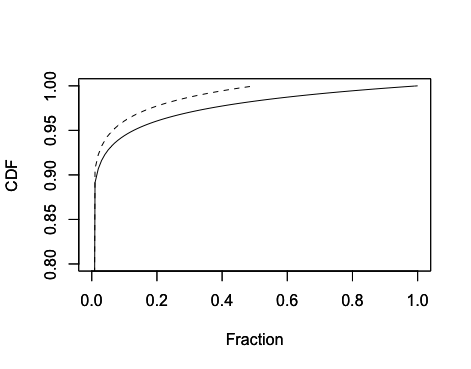
\includegraphics[scale = 0.6]{prob2_cdf.png}
			\caption{Cumulative distribution of $D$ and $L$}
			\label{fig:prob2-cdf}9
		\end{figure}
		\item  %% (b)
		Let $x$ denote the lowest attachment point such that the probabilities
		of the tranche above that point experiencing any principal loss is $p$.
		Since cumulative distribution function is monotonically increasing,
		probability such that fraction of loss for CLO is greater than $x$ is
		equal to $p$. (i.e. $Prob(L > x) = p$) Solving the equation, $x$ is
		derived as follows.
		\begin{equation*}
			\begin{aligned}
				Prob(L > x)	= p	\\
				1 - \left( \frac{x}{1 - R} \right)^{\frac{b}{a}}	= p	\\
				x = (1 - R) \times (1 - p)^{\frac{a}{b}}
			\end{aligned}
		\end{equation*}
		Table \ref{tab:prob2-attachment} shows the lower attachments for
		each tranche calculated by using the equation above. From the table
		about 50\% of loans consists of AAA ratings.
		\begin{table}[ht]
\centering
\begin{tabular}{@{}ccc@{}}
\toprule
Tranches & Probabilities & Attachments(Lower) \\ \midrule
AAA      & 0.05\%        & 0.490              \\
AA       & 0.20\%        & 0.462              \\
A        & 1\%           & 0.334              \\
BBB      & 2\%           & 0.223              \\
BB       & 7.50\%        & 0.022              \\
Unrated  &               & 0.000              \\ \bottomrule
\end{tabular}
\caption{Attachment of each tranche}
\label{tab:prob2-attachment}
\end{table}

		\item  %% (c)
		Let $N$ denote the notional amount of CLO as a whole. Then, face value
		of each tranche is equal to proportion of each tranche times $N$.
		Assuming interests are paid annually, interest payment for each tranche
		is calculated.
		Table \ref{tab:prob2-loan} represents annual interest payment for each
		tranche.
		\begin{table}[ht]
\centering
\begin{tabular}{@{}cccc@{}}
\toprule
Tranches & Proportion & Interest         & Payment                      \\ \midrule
AAA      & 0.51       & LIBOR + 0.25\%   & $-0.51 \times N \times (LIBOR + 0.25\%)$ \\
AA       & 0.03       & LIBOR + 0.5\%    & $-0.03 \times N \times (LIBOR + 0.5\%)$  \\
A        & 0.13       & LIBOR + 1.25\%   & $-0.13 \times N \times (LIBOR + 1.25\%)$ \\
BBB      & 0.11       & LIBOR + 2.5\%    & $-0.11 \times N \times (LIBOR + 2.5\%)$  \\
BB       & 0.20       & LIBOR + 4\%      & $-0.20 \times N \times (LIBOR + 4\%)$    \\
Sum      & 0.98       &                  & $-0.98 \times N \times LIBOR + N \times 1.38\%$ \\ \bottomrule
\end{tabular}
\caption{Annual payment of each tranche}
\label{tab:prob2-loan}
\end{table}

		Since we assumed that the bottom level tranche is entirely wiped out,
		and the loss is amortized equally, issuer will get
		$0.98 \times N \times (LIBOR + 4\%)$ amount of interest payment
		at each year. Therefore, the interest margin is calculated as
		$-0.98 \times N \times LIBOR + N \times 1.38\% -
			0.98 \times N \times (LIBOR + 4\%) = N \times 2.54\%$.
		Therefore, interest margin for this scenario is 2.54\% per year.
	\end{enumerate}
\end{homeworkProblem}

%----------------------------------------------------------------------------------------
%	PROBLEM 3
%----------------------------------------------------------------------------------------
\begin{homeworkProblem}
	\begin{enumerate}[(a)]
		\item  %% (a)
		Assume the swap matuares at $T$.
		In order to derive $V(S_t, t, \varphi_0)$, it needs to derive each leg
		of swap first. Since bank pays $\varphi$ dollars continuously,
		present value of the leg is evaluated as
		$\varphi \int_t^T e^{-r_d s}ds = \varphi (-\frac{1}{r_d}) e^{-r_d s}
			\rvert^T_t = \frac{\varphi}{r_d}e^{-r_d t}(1 - e^{-r_d(T - t)})$.
		Similarly, present value of the foreign currency leg is evaluated as
		$S_t \int_t^T e^{-r_f s}ds = S_t (-\frac{1}{r_f}) e^{-r_f s}
			\rvert^T_t = \frac{S_t}{r_f}e^{-r_f t}(1 - e^{-r_f(T - t)})$.
		Equating both equations, $\varphi_0$ is calculated as follows.
		\begin{equation*}
			\begin{aligned}
				\frac{\varphi_0}{r_d}(1 - e^{-r_d T})
					&= \frac{S_0}{r_f}(1 - e^{-r_f T})	\\
				\Rightarrow \varphi_0 &= \frac{S_0 r_d}{r_f}
					\left( \frac{1 - e^{-r_f T}}{1 - e^{-r_d T}} \right)	\\
					&= \frac{0.01}{0.05}
						\left( \frac{1 - e^{-0.05 \times 5}}
						 	{1 - e^{-0.01 \times 5}}\right)	\\
					&= 0.9071
			\end{aligned}
		\end{equation*}
		\item  %% (b)
		Since there is no collateral, we can assume that there is no recovery if
		the counterparty is default.
		Therefore, CVA of the contract is derived as follows.
		\begin{equation*}
			\begin{aligned}
				CVA	&= \int_0^T e^{-r_d t} 1_{\text{\{c/p defaults at t\}}}
					\max(V_t, 0) dt	\\
					&= \int_0^T e^{-r_d t} \lambda_t e^{-\int_0^t \lambda_u du}
						\max \left( \frac{S_t}{r_f} e^{-r_f t}(1 - e^{-r_f (T- t)})
							 - \frac{\varphi_0}{r_d} e^{-r_d t} (1 - e^{-r_d (T - t)}), 0 \right)dt
			\end{aligned}
		\end{equation*}
		In order to execute simulation, I discretized the integral as follows.
		\begin{equation*}
			\begin{aligned}
				CVA	&= \sum_{i = 0}^{M} \left[ e^{-r_d(i\Delta t)}
					\lambda_i e^{-\sum_{j = 0}^i \lambda_j \Delta t} \right. \\
					& \left. \times \max \left( \frac{S_i}{r_f} e^{-r_f (i \Delta t)}(1 - e^{-r_f (T - i \Delta t)})
						 - \frac{\varphi_0}{r_d} e^{-r_d (i \Delta t)} (1 - e^{-r_d (T - i \Delta t)}), 0 \right) \Delta t
				 \right]	\\
				M \Delta t &= T	\\
				\lambda_i	&= \lambda_{i - 1} \times
					\exp[(b_{\lambda}^Q - 0.5\sigma_{\lambda}^2)\Delta t
							+ \sigma_{\lambda} \sqrt{\Delta t} \phi_1]	\\
				S_i	&= S_{i - 1} \times
					\exp[(r_d - r_f - 0.5 \sigma_S^2)\Delta t
							+ \sigma_S \sqrt{\Delta t} \phi_2]	\\
				\begin{pmatrix}
					\phi_1	\\ \phi_2
				\end{pmatrix}
				&\sim
				N\left(
					\begin{pmatrix}
						0	\\	0
					\end{pmatrix}
					,
					\begin{pmatrix}
						1	& \rho	\\	\rho & 1
					\end{pmatrix}
				\right)
			\end{aligned}
		\end{equation*}
		By simulating 5000 times with $M = 450$ for $\rho = 0, 0.1, 0.2 \dots
		1.0$, and using given parameters, CVA was calculated at each correlation.
		Figure \ref{fig:prob3-cva} shows CVA at each correlation.
		\begin{figure}[ht]
		\centering
			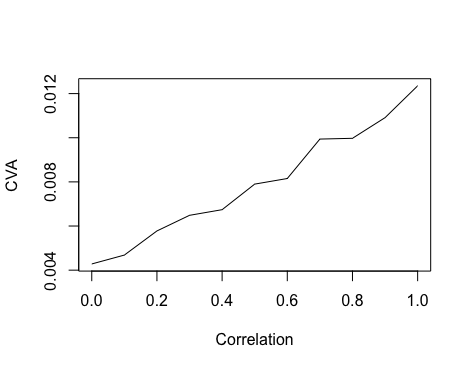
\includegraphics[scale = 0.6]{prob3_cva.png}
			\caption{CVA at each correlation}
			\label{fig:prob3-cva}
		\end{figure}
		From the figure, we can discover that CVA increases as correlation
		increases. Since the bank earns more money if exchange rate increases,
		if default intensity is highly correlated with exchange rate,
		expected amount of position value when counterparty defaults will be
		higher. That's why CVA increases as correlation increases.
		Since CVA at $\rho = 0.5$ is calcuated as 0.789921\%, if notional value
		of swap is 1 billion, CVA is calculated as about 7.899 million dollars.
	\end{enumerate}
\end{homeworkProblem}

%----------------------------------------------------------------------------------------
%	PROBLEM 4
%----------------------------------------------------------------------------------------
\begin{homeworkProblem}
	\textbf{I disagree.} RMBS itself is not a main reason for subprime crisis.
	The main reason was re-securitized product. Actually, about 80\% of pool
	was AAA tranche. Therefore, although cumulative default rate on the pool
	reached 40\%, investors would not have experienced extreme loss.
\end{homeworkProblem}

%----------------------------------------------------------------------------------------
%	PROBLEM 5
%----------------------------------------------------------------------------------------
\begin{homeworkProblem}
	\begin{enumerate}[(a)]
		\item  %% (a)
		For each $r \in \{0.01, 0.02 \dots 0.16\}$, NPV was calculated by
		simulating 10,000 paths. Principal amount was assumed to be 100.
		Figure \ref{fig:prob5-npv} shows NPV of MBS
		when $b = -30$, and $b = 0$, respectively.
		We can find out that NPV decreases as initial interest rate increases
		as future cash flows is highly discounted.
		\begin{figure}
		\centering
			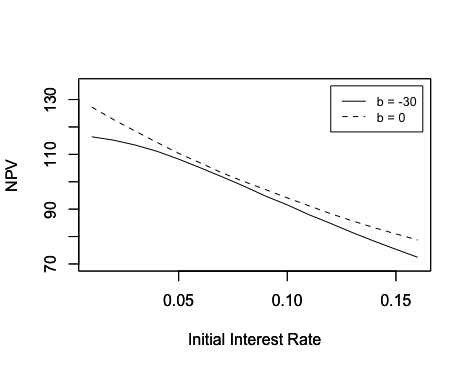
\includegraphics[scale = 0.6]{prob5_plot1.png}
			\caption{NPV at each $r$}
			\label{fig:prob5-npv}
		\end{figure}
		\item  %% (b)
		From Figure \ref{fig:prob5-npv}, it can be discovered that NPV when
		$b = 0$ is always higher then when $b = -30$, and it has relatively
		linear shape though NPV when $b = -30$ is relatively concave.
		Figure \ref{fig:prob5-diff} shows the absolute value of difference
		between NPV when $b = -30$ and $b = 0$, we can find that difference
		has a convex shape, which occurs because NPV when $b = -30$ has a
		concavity.
		\begin{figure}
		\centering
			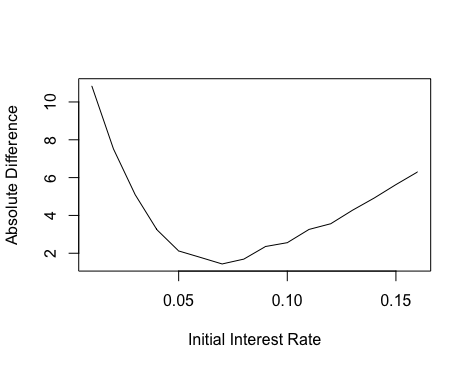
\includegraphics[scale = 0.6]{prob5_plot2.png}
			\caption{Absolute difference of NPV}
			\label{fig:prob5-diff}
		\end{figure}
		\item  %% (c)
		In this case, factors which affects NPV of MBS are amount of prepayment
		and discount factor. Prepayment decreases future interest payments of
		the pool, and discount factor affects time value of money. They have
		trade-off because prepayment decreases future cash flow, but it is
		discounted less.
		When interest rate is low, prepayment has a negative
		effect because interest payments decreases, and discount factor affects
		a little. However, if interest rate is high, prepayment has a positive
		effect to NPV because time value of money dominates NPV.
		From this perspective, if $\pi$ is sensitive to interest rate, it has
		negative effect because higher sensitivity means higher prepayment
		if interest rate is low, and lower prepayment if interest rate is higher.
		Also, from this reason concavity of NPV occurs, and if sensitivity
		gets higher, NPV will be more concave.
		\item  %% (d)
		It needs to sell more the bond in (b) if price goes down.
		From the perspective of hedging interest rate risk, price of MBS
		goes down if interest rate gets higher. From Figure \ref{fig:prob5-npv},
		we can easily find that the bond (a) gets more sensitive to interest
		rate if its price goes down, whereas sensitivity of bond (b) is relatively
		stable. It means that in order to match sensitivity of long position
		and short position, it needs to sell more bond (b) if price goes down.
	\end{enumerate}
\end{homeworkProblem}
\end{document}
